% !TeX root = ../main.tex

\section{Results}

\subsection{Statistical analysis of spacing distribution}

First,we calculate the first 10000 eigenvalues of each system by diagonalizing the sparse matrix that we obtained applying the FDM \ref{eq:sparse_matrix}. Then, with those arrays, we compute a new one that has the spacing distribution between consecutive eigenvalues, this is $s = E_{i+1} - E_i$. 
Since the Poisson and Wigner distributions are defined in the normalized space, we must normalize then the spacing by doing $s \rightarrow s/<s>$.

Finally, we plot an histogram of the normalized spacing between adjacent eigenvalues, as it follows:
\begin{figure}[H]
    \centering
    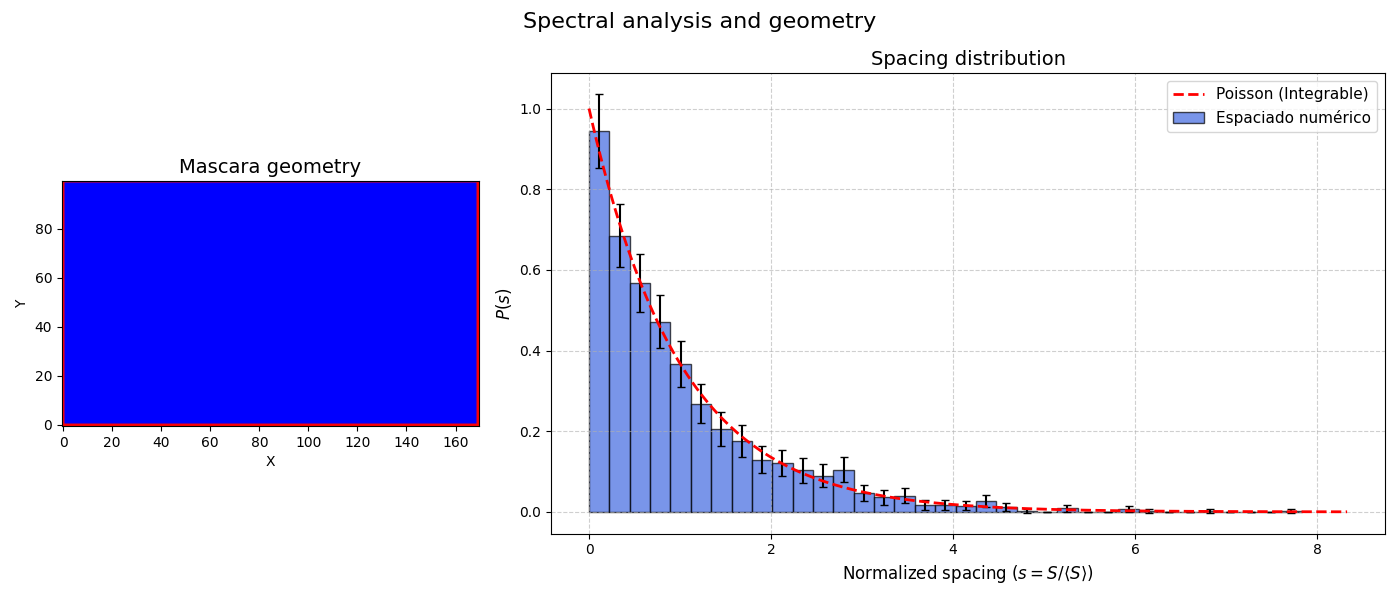
\includegraphics[width=\textwidth]{img/170x100_distr_r.png}
    \caption{Blue bars represent the histogram spacings, with associated errorbars that follows a counting Poisson error in a $95\% (\pm 2\sigma)$ confidence interval. The red line is the expected Poisson distribution \ref{eq:Poisson_dist}. The considered system is the rectangle mascara.}
    \label{fig:poisson_distribution}
\end{figure}

\begin{figure}[!ht]
    \centering
    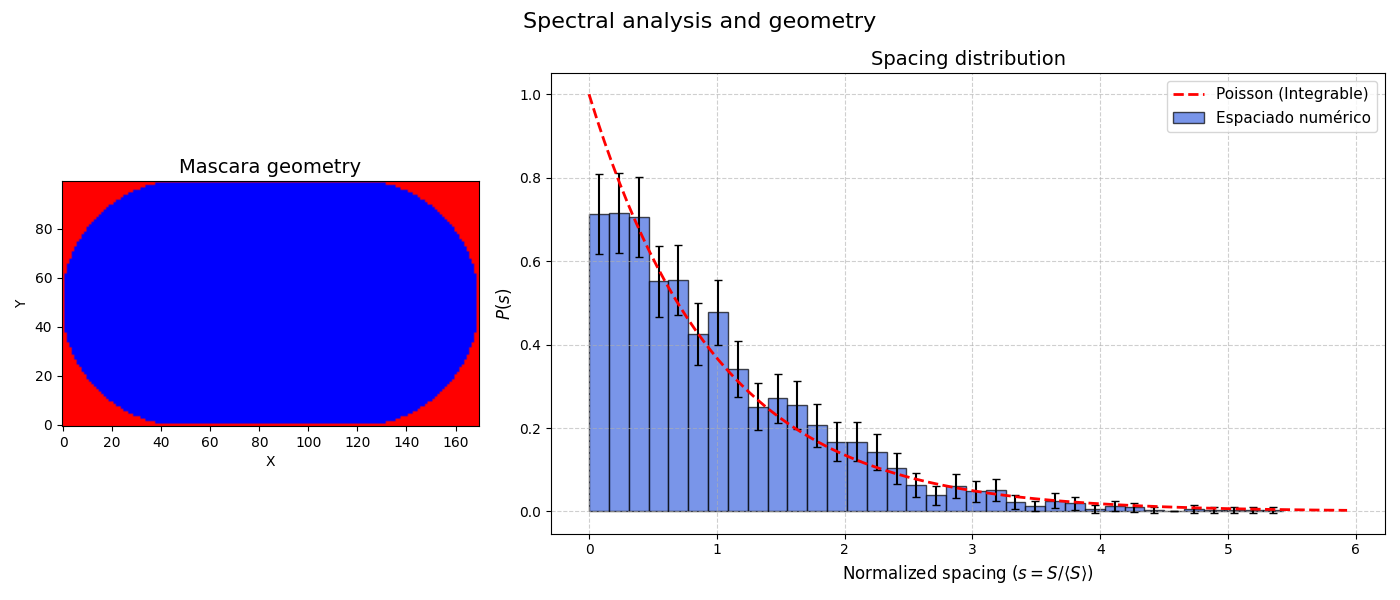
\includegraphics[width=\textwidth]{img/170x100_distr_c.png}
    \caption{Blue bars represent the histogram spacings, with associated errorbars that follows a counting Poisson error in a $95\% (\pm 2\sigma)$ confidence interval. The red line is the distribution that fits the better the tendency of the histogram. The considered system is the complete billiard.}   
    \label{fig:poisson_distribution_stadium}
\end{figure}

\begin{figure}[!ht]
    \centering
    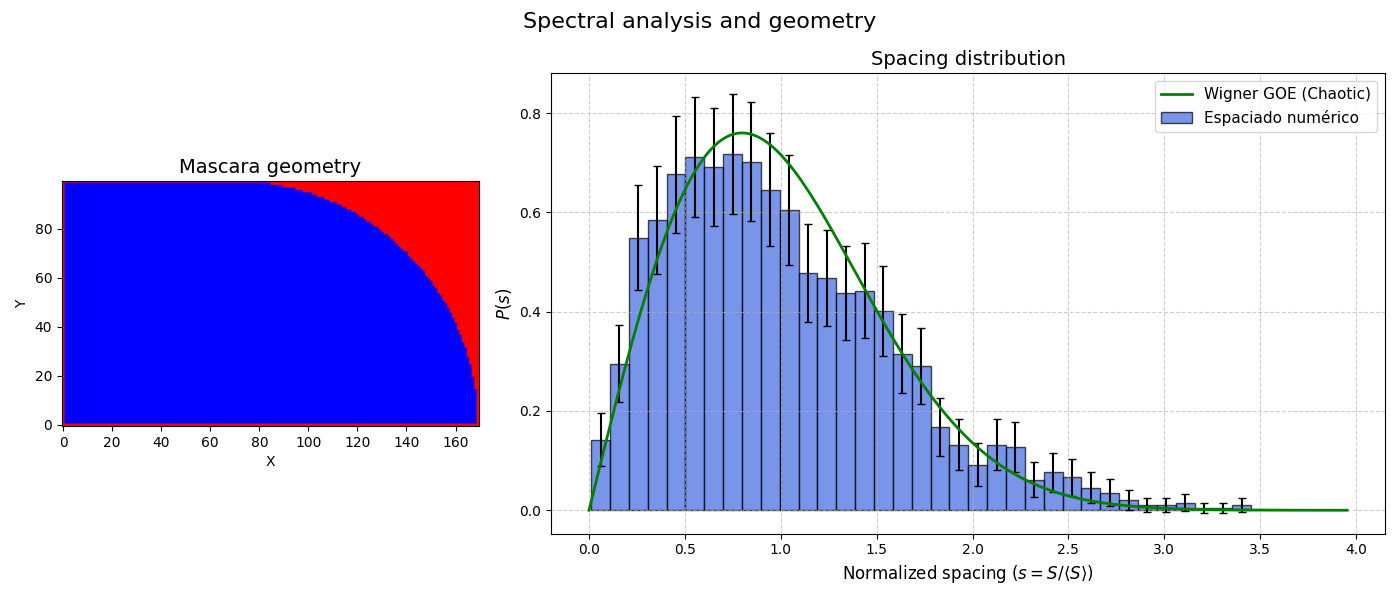
\includegraphics[width=\textwidth]{img/170x100_distr_qc.png}
     \caption{Blue bars represent the histogram spacings, with associated errorbars that follows a counting Poisson error in a $95\% (\pm 2\sigma)$ confidence interval. The green line is the expected WD distribution \ref{eq:Wigner-Dyson_dist} for a non-integrable system. The considered system is a quarter of the billiard.}    
    \label{fig:wigner_dyson_distribution}
\end{figure}

As expected, we can clearly see in \autoref{fig:poisson_distribution} that the spacing distribution for the integrable rectangle follows a Poisson distribution. This graphic shows how this systems, even if it is integrable, that their eigenvalues are not correlated, then the probability of finding two eigenvalues close to each other is high ($P(s) \rightarrow 1$ when $s \rightarrow 0$). 

Also, in the case of the non-integrable billiard (the complete stadium showed in  \autoref{fig:poisson_distribution_stadium}), we can see that it also follows a near Poisson distribution, due to the symmetries of the system. This symmetries make the system to have four pairs of solutions, then, the degenerate levels will increase the probability of finding two eigenvalues close to each other, even if the system is non-integrable.\\


On the other hand, if we eliminate the $x-axis$ and $y-axis$ symmetries, having just a quarter of the stadium as we see in \autoref{fig:wigner_dyson_distribution}, it is noticeable that the spacing distribution for the non-integrable billiard follows a Wigner-Dyson distribution. In this case, the opposite happens: the system may seem chaotic, but its eigenvalues are correlated, in a way that makes them repel each other or, in other words, the probability of finding two near-degenerate eigenvalues is very low ($P(s) \rightarrow 0$ when $s \rightarrow 0$). \cite{Nakayama2020}


\subsection{High-energy states visualization}

To determine the chaocity of the system, we must look at high-energy states, and compare them to the non-chaotic system. This is due to the fact that, in the low-energy states, the eigenvectors may seem like those of a string, therefore, they don't contain the necessary information to see if the system is chaotic or not. We then plot the probability density of some of the high-energy states for both systems. 

\begin{figure}[!ht]
    \centering
    % Primera imagen
    \begin{subfigure}[b]{0.9\textwidth}
        \centering
        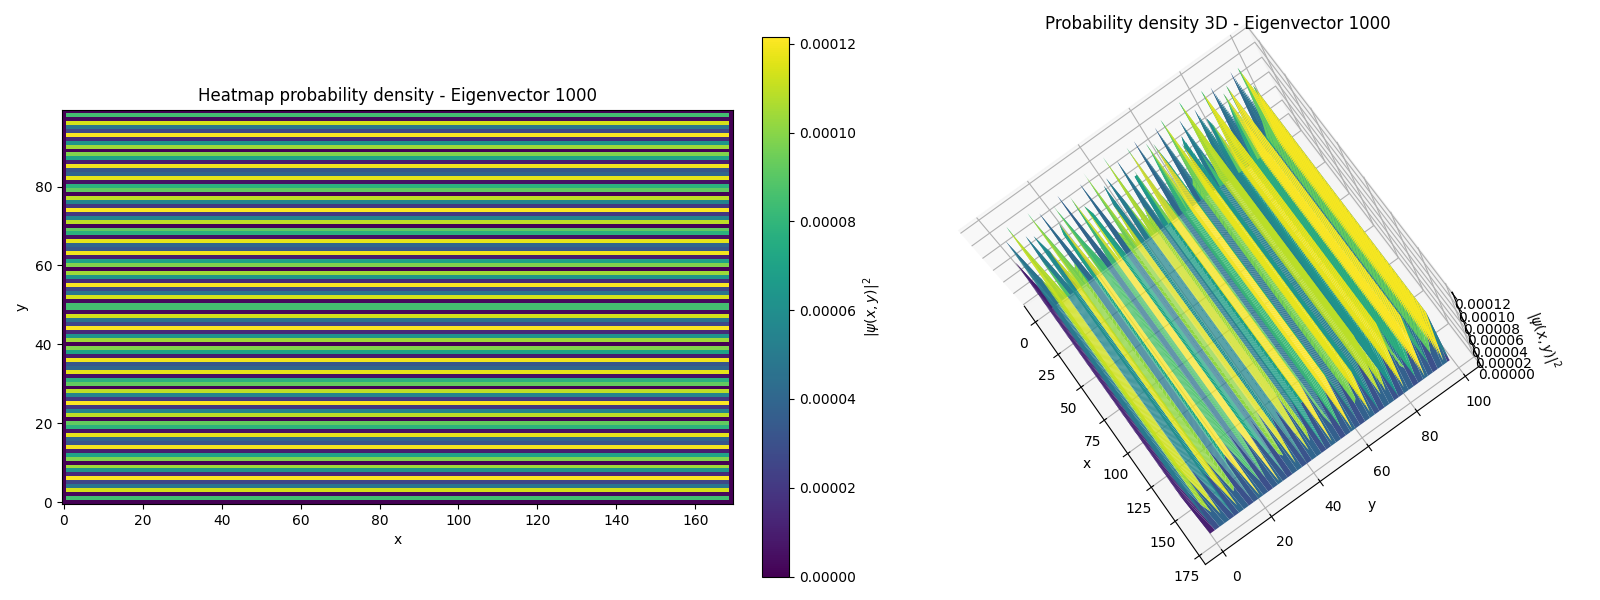
\includegraphics[width=\textwidth]{img/dens_prob_r_975.png} %el valor del nombre de la imagen no  corresponde al que es porque lo cambiamos a ultima hora par que se viera mejor. Este es para el 1000
        \caption{Probability density for the eigenvalue 1000.}
        \label{fig:rectangle_975}
    \end{subfigure}
    
    \vspace{1em} % Espacio vertical entre imágenes
    
    % Segunda imagen
    \begin{subfigure}[b]{0.8\textwidth}
        \centering
        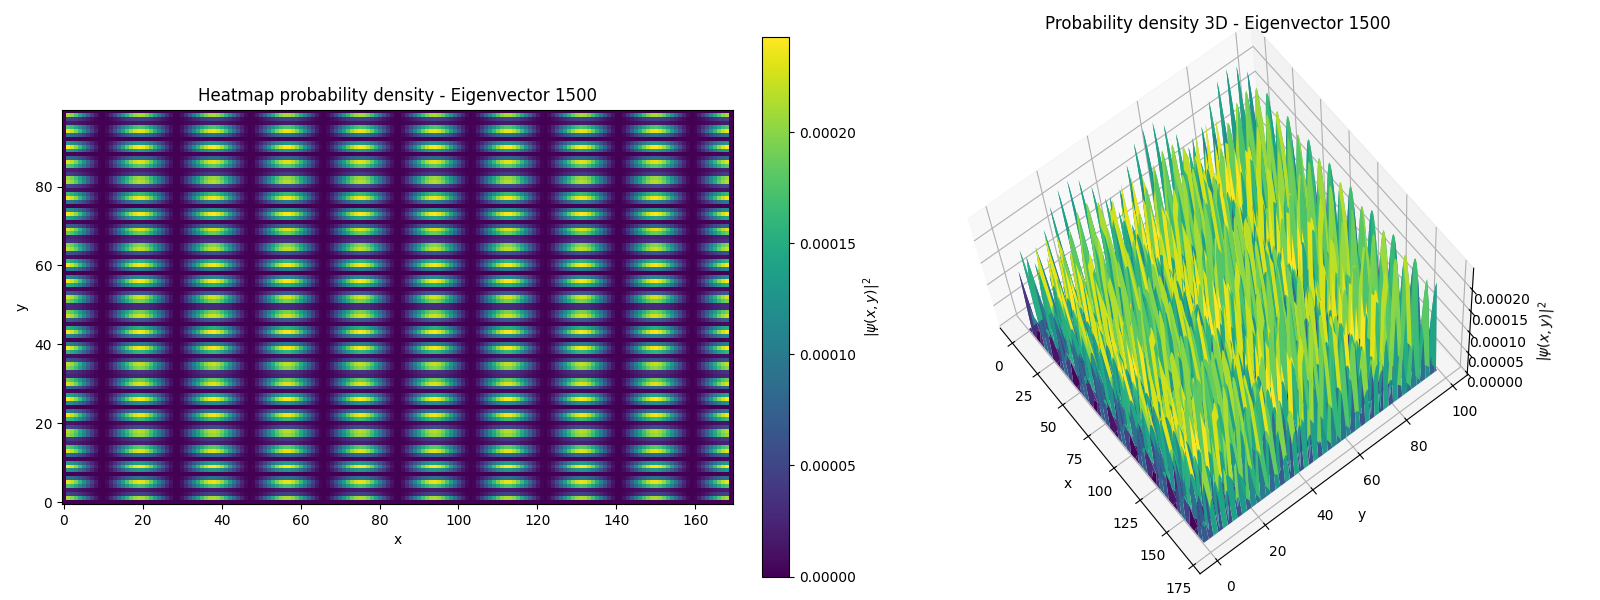
\includegraphics[width=\textwidth]{img/dens_prob_r_985.png}
        \caption{Probability density for the eigenvalue 1500.}
        \label{fig:rectangle_985}
    \end{subfigure}
    
    \vspace{1em} % Espacio vertical entre imágenes
    
    % Tercera imagen
    \begin{subfigure}[b]{0.8\textwidth}
        \centering
        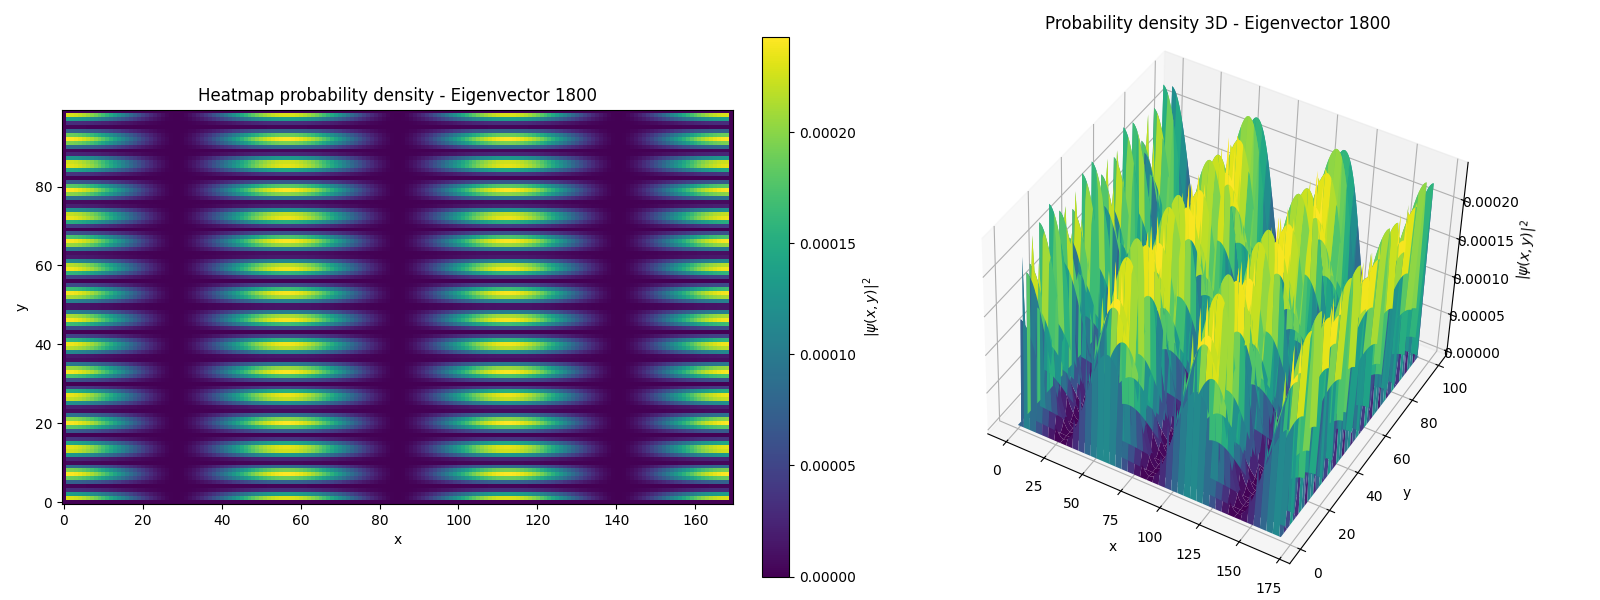
\includegraphics[width=\textwidth]{img/dens_prob_r_995.png}
        \caption{Probability density for the eigenvalue 1800.}
        \label{fig:rectangle_995}
    \end{subfigure}
    
    \caption{Visualization of various of the high-energy states for the \textbf{integrable rectangle}. In the left, it shows the heatmap of the probability density for the eigenvalues 1000, 1500, and 1800; in the right, the same is shown, but in 3D, having axis x and y, and the third dimension represents the probability density.}
    \label{fig:dens_prob_r}
\end{figure}



\begin{figure}[!ht]
    \centering
    % Primera imagen
    \begin{subfigure}[b]{0.8\textwidth}
        \centering
        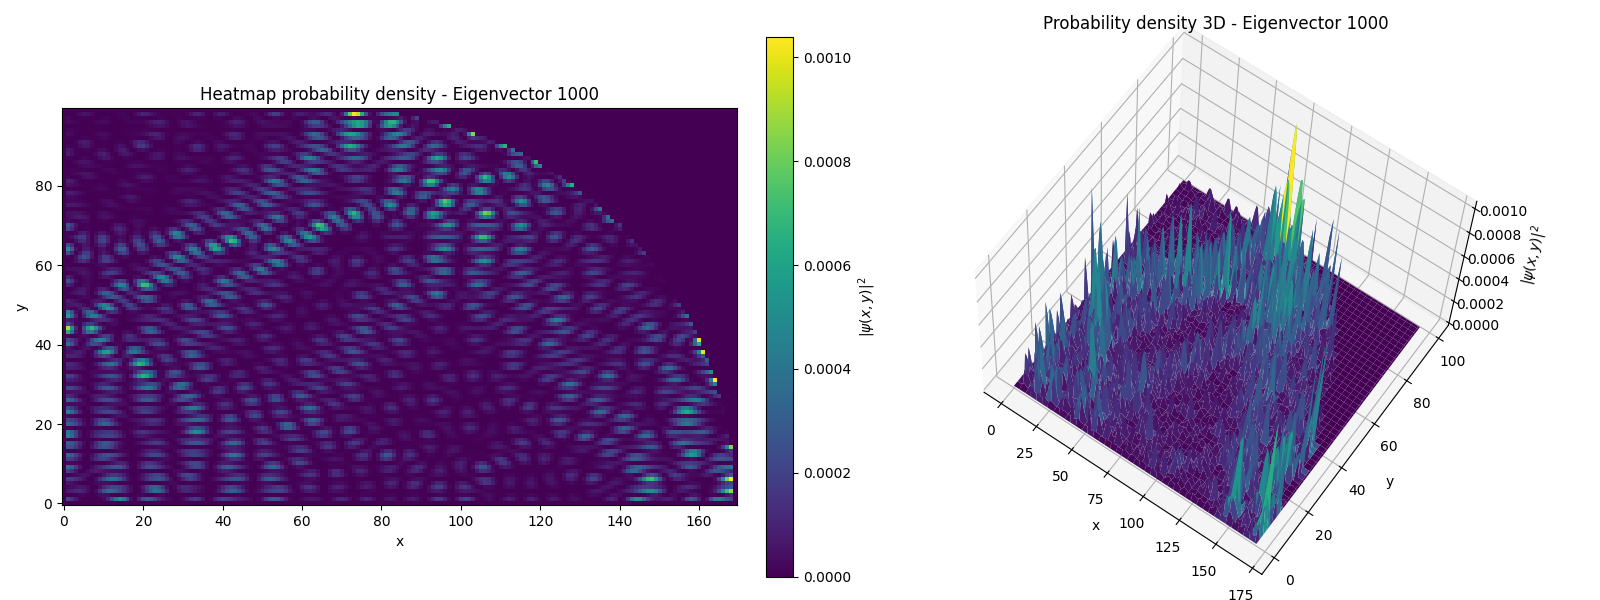
\includegraphics[width=\textwidth]{img/dens_prob_qc_975.png}
        \caption{Probability density for the eigenvalue 1000.}
        \label{fig:qc_975}
    \end{subfigure}
    
    \vspace{1em} % Espacio vertical entre imágenes
    
    % Segunda imagen
    \begin{subfigure}[b]{0.8\textwidth}
        \centering
        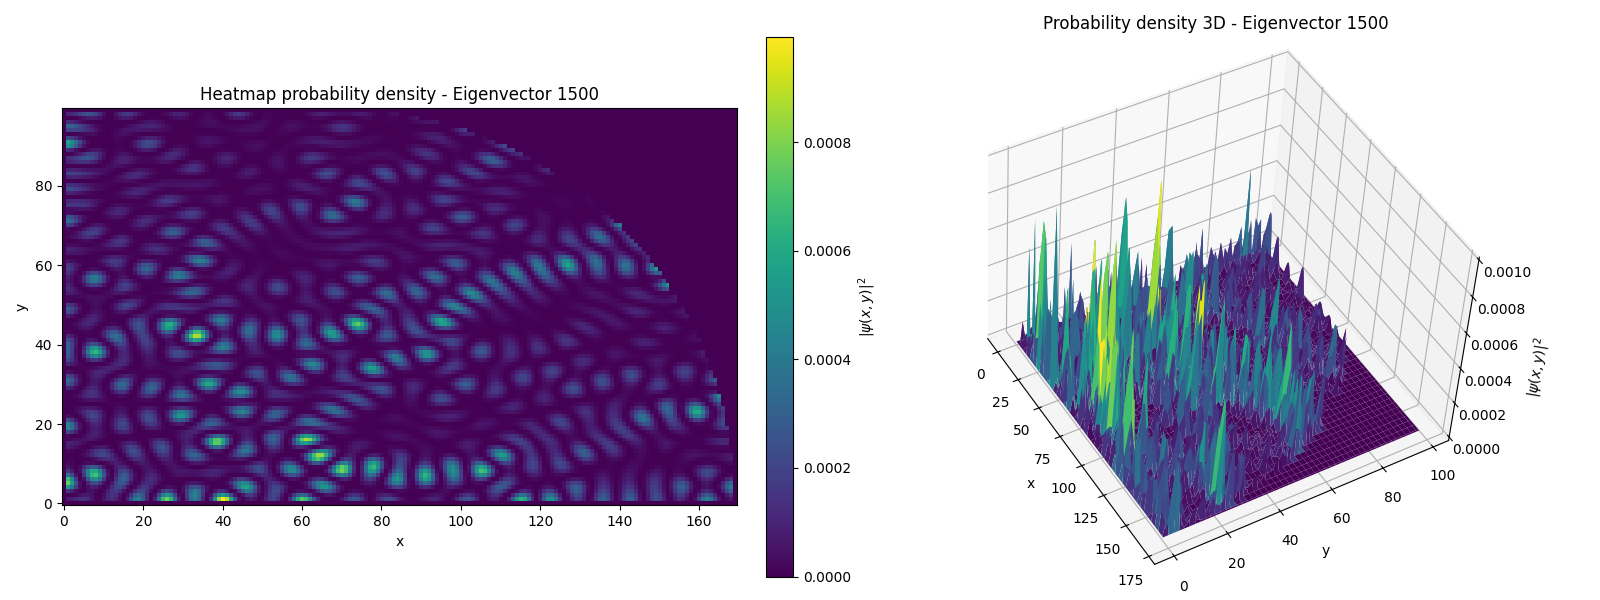
\includegraphics[width=\textwidth]{img/dens_prob_qc_985.png}
        \caption{Probability density for the eigenvalue 1500.}
        \label{fig:qc_985}
    \end{subfigure}
    
    \vspace{1em} % Espacio vertical entre imágenes
    
    % Tercera imagen
    \begin{subfigure}[b]{0.8\textwidth}
        \centering
        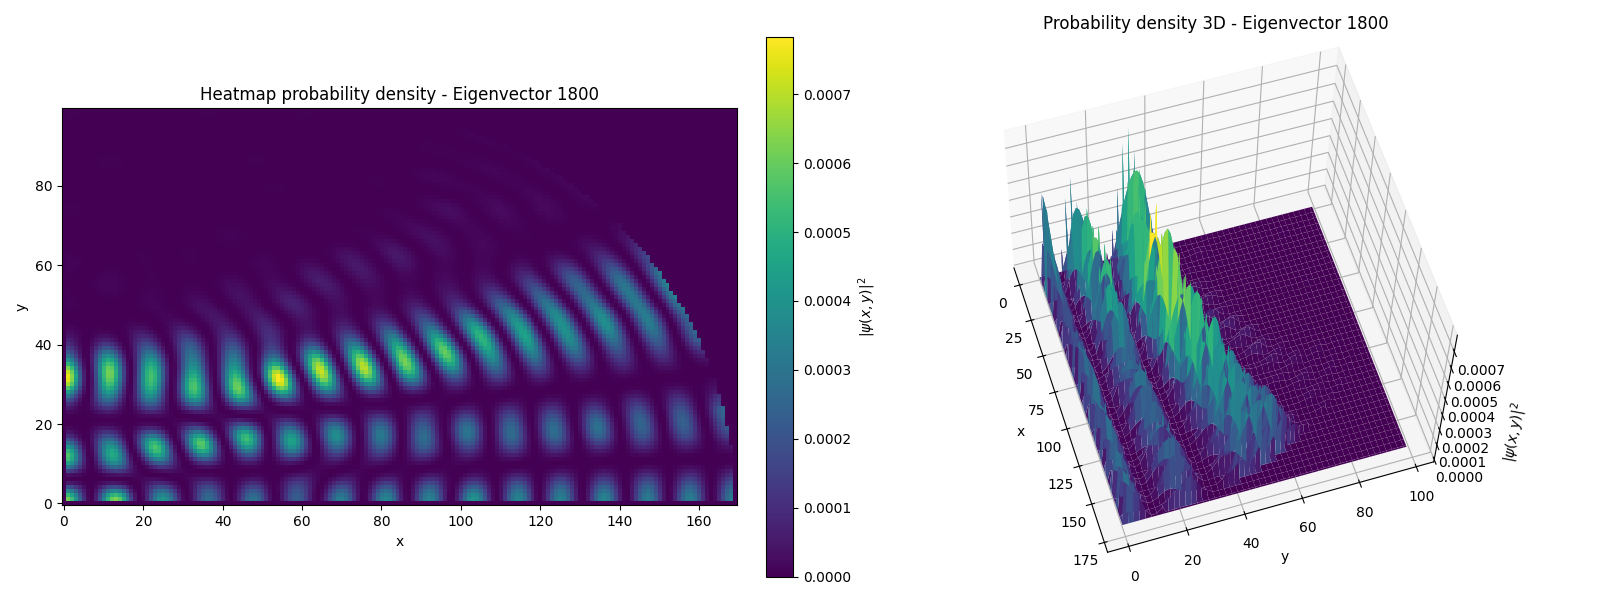
\includegraphics[width=\textwidth]{img/dens_prob_qc_995.png}
        \caption{Probability density for the eigenvalue 1800.}
        \label{fig:qc_995}
    \end{subfigure}
    
    \caption{Visualization of various of the high-energy states for the \textbf{non-integrable quarter billiard}. In the left, it shows the heatmap of the probability density for the eigenvalues 1000, 1500, and 1800; in the right, the same is shown, but in 3D, having axis x and y, and the third dimension represents the probability density.}
    \label{fig:dens_prob_qc}
\end{figure}


The three graphics of \autoref{fig:dens_prob_r} show the probability density for three of the high-energy states of the integrable rectangle.We see that the patterns are very regular, and they look like the fundamental modes of a string, with nodes and antinodes. We can determine then that this system is not chaotic, as expected, since there are periodic patterns in the probability density.

In contrast, the same eigenvalues are shown for the non-integrable quarter billiard in \autoref{fig:dens_prob_qc}. In this system, the probability density is not random or uniformly distributed, but it shows some patterns that are not regular, and they don't look like the fundamental modes of a string.\\
This is a striking result: in a classically chaotic system, one would expect an erratic way of filling the space, without any specific path or visual pattern. Yet, as seen in \autoref{fig:dens_prob_qc}, certain high-energy eigenstates show a clear concentration of probability density along specific curves in this quarter of the billiard. \\ 

If we reverse the same reasoning that we stated to divide the complete billiard in just a quarter to eliminate the symmetries, now we can take advantage of this symmetries to visualize better this trajectory along the billiard, since it will be a closed trajectory and, therefore, it's directly comparable to a classical orbit. 

\begin{figure}[!ht]
    \centering
    
    % Segunda imagen
    \begin{subfigure}[b]{0.7\textwidth}
        \centering
        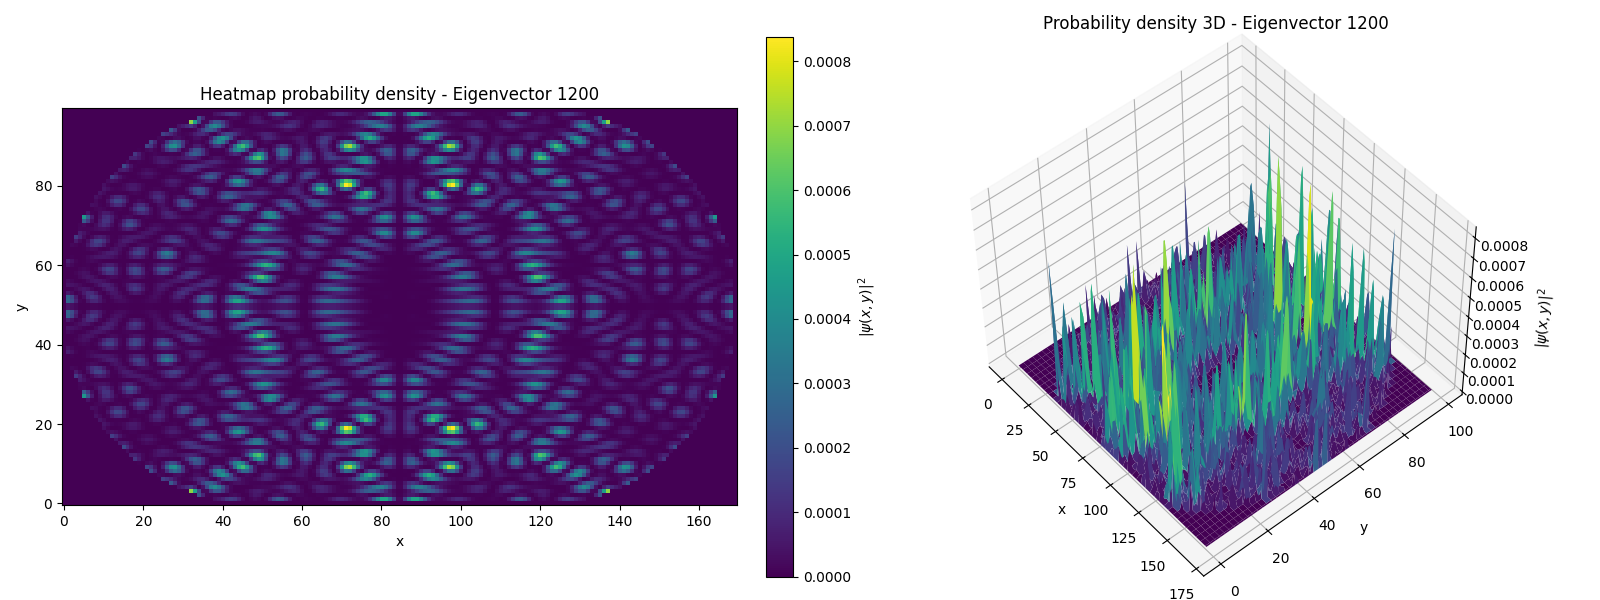
\includegraphics[width=\textwidth]{img/dens_prob_c_1200.png}
        \caption{Probability density for the eigenvalue 1200.}
        \label{fig:qc_1200}
    \end{subfigure}
    
    \vspace{1em} % Espacio vertical entre imágenes
    
    % Tercera imagen
    \begin{subfigure}[b]{0.7\textwidth}
        \centering
        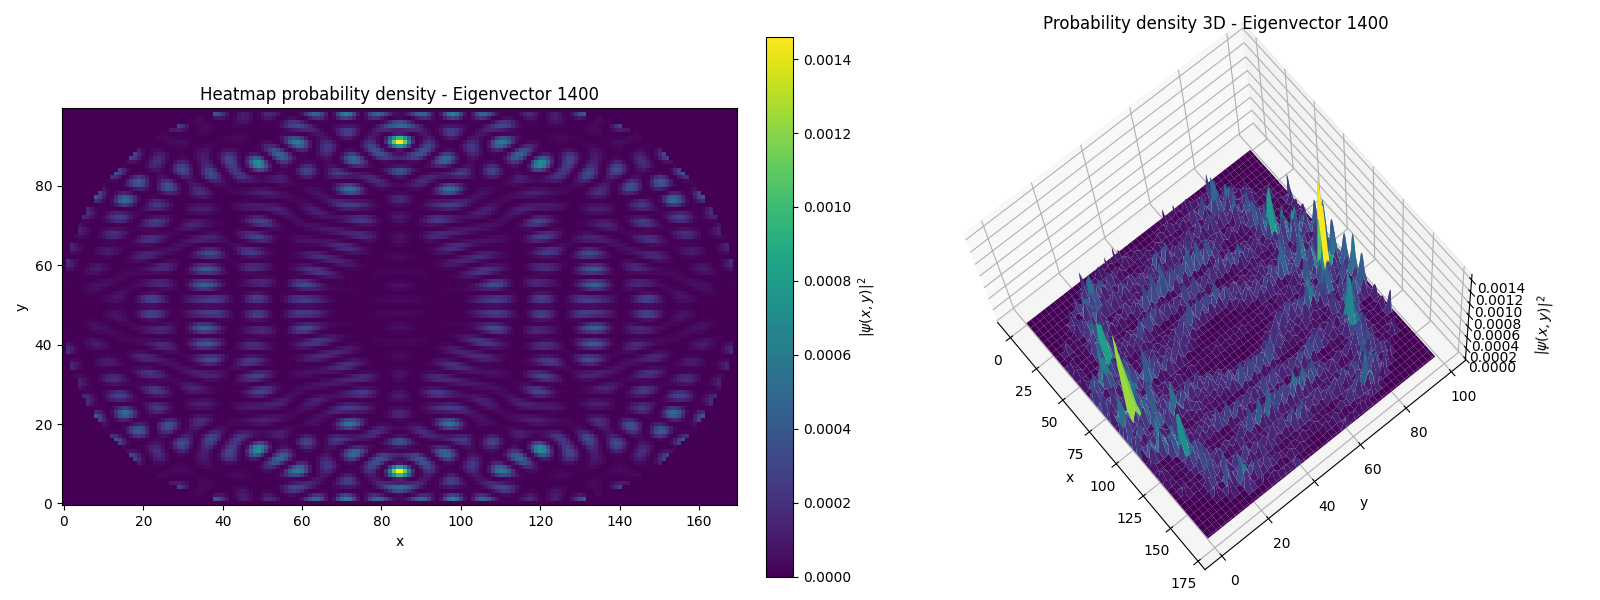
\includegraphics[width=\textwidth]{img/dens_prob_c_1400.png}
        \caption{Probability density for the eigenvalue 1400.}
        \label{fig:qc_1700}
    \end{subfigure}

    \vspace{1em}

    % Primera imagen
    \begin{subfigure}[b]{0.7\textwidth}
        \centering
        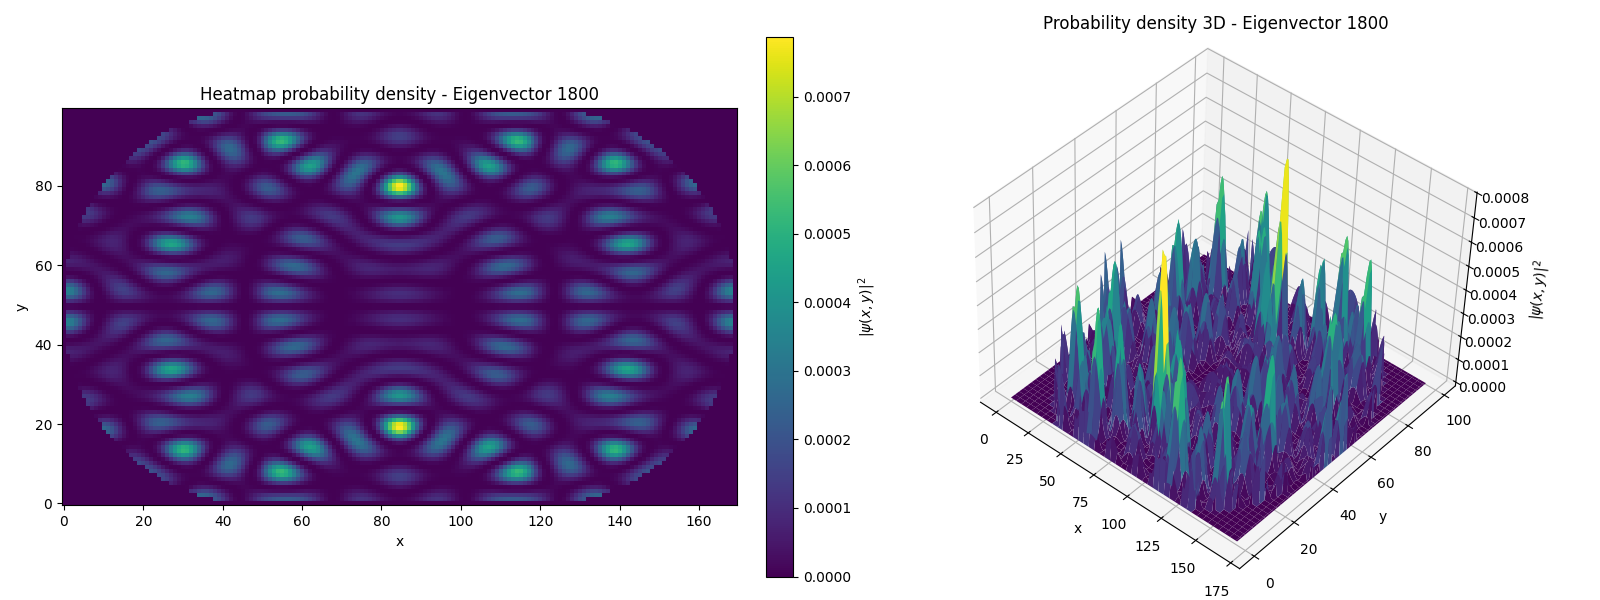
\includegraphics[width=\textwidth]{img/dens_prob_c_800.png}
        \caption{Probability density for the eigenvalue 1800.}
        \label{fig:qc_800}
    \end{subfigure}
    
    \caption{Visualization of various of the high-energy states for the \textbf{non-integrable complete billiard}. In the left, it shows the heatmap of the probability density for the eigenvalues 1200, 1400, and 1800 of the billiard. In the right, the same is shown, but in 3D, having axis x and y, and the third dimension represents the probability density.}
    \label{fig:dens_prob_c}
\end{figure}

Now, in \autoref{fig:dens_prob_c} we can see for those cases that this closed trajectory ressemble of a classical one. This is what is known as \textbf{'Quantum Scars'}, and they correspond to the unstable periodic orbits of the classical system.  The origin of quantum scars lies in wave interference: the quantum wavefunction can constructively interfere along the path of a periodic orbit, even if that orbit is unstable (which is the case, because in this system, another initial condition will make that the final result is totally different). 

It's important to note that we'd only uploaded the files that we'd see representative. Any other state can be checked in the provided code in the github. \cite{PCSProject}


\subsubsection{Ergodicity in the quantum system}

A system is said to be ergodic when, after evolving for a sufficiently long time, a single trajectory visits every region of the accesible phase space. According to Shnirelman's theorem (also known as the quantum ergodicity theorem), this classical ergodicity is reflected in the corresponding quantum system: for almost all high-energy eigenstates, the probability density becomes equidistributed over the spatial domain in the semiclassical limit. 

This theorem is showed in our figures: the rectangular system shows regions with zero probability of the particle to be in that position, as we can see at any example of the \autoref{fig:dens_prob_r}. Meanwhile, the quantum system has a non zero probability in every point of the space. \\
If we imagine the system as a ball hitting the edges of the surface and bouncing during a long time, the ball will never cross certain areas in the case of the rectangle, but, in the billiard, eventually it will have crossed the entire surface at leas one time. 

At last, it's interesting to discerne the quantum scars from the ergodicity theorem. Although Shnirelman's theorem predicts that the probability density of high-energy eigenstates in a chaotic system should eventually become equidistributed, the presence of quantum scars introduce a nuance to this ergodicity. \\
This phenomenom is explained with the Gutzwiller's Trace Formula, which relates the quantum density of states to a summation over all classical periodic orbits: eigenvalues emerge as singularities where wave phases interfere, as we said, constructively along these paths. Consequently, while the system tends toward ergodicity in the semiclassical limit, these scars represent a visual suppression of classical chaos. \cite{WikipediaQuantumScar}